\chapter{訓練環境}
\section{OpenAI Gym}
 Gym 是用於開發和比較強化學習算法的工具包,他不對agent的結構做任何假設,並且與任何數據計算庫兼容,而可以用來制定強化學習的算法。這個環境具有共享的介面,使我們能用來編寫常規算法,也就能教導agents如何步行到玩遊戲。\\[6pt]

\section{Pong}
 取自 1977年發行的一款家用遊戲機ATARI 2600中的遊戲,內建於Gym,這是一個橫向的乒乓遊戲,左方是遊玩者,右邊由使用者操控或是由訓練的機器控制(圖.\ref{fig.pong})。\\
\begin{figure}[hbt!]
\begin{center}
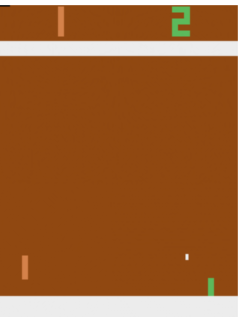
\includegraphics[height=8cm]{pong_gym}
\caption{\Large ATARI Pong}\label{fig.pong}
\end{center}
\end{figure} 
 
\section{Pong from pixels}
Pong的遊戲是簡單的強化學習中,很好的例子,在ATARI 2600版本中,我們會控制右邊邊的操縱板(左邊由電腦控制)。遊戲的運行方式如下:我們收到一個圖像幀(一個210x160x3 byte數組(從0到255的整數給出像素值)),然後決定是否要向上或向下移動操縱板(即二進制選擇)。每次選擇之後,遊戲模擬器就會執行動作並給予我們獎勵:如果球超過了對手,則為+1獎勵;如果我們錯過球,則為-1獎勵;否則為0。當然,我們的目標是移動球拍,以便獲得很多獎勵。\\

\newpage